\chapter{Konzept}
\label{konzept}

Das Ziel der Webanwendung ist die schnelle und einfache Bildung von Gruppen in Echtzeit. Das gewählte Konzept sieht als oberste Element den Raum vor. Der Raum kann bspw. im Kontext der Universität als das Äquivalent zu einer Vorlesung betrachtet werden. Die Anwendung erlaubt es jedem Benutzer beliebig viele Räume zu erstellen oder beliebig vielen bereits vorhandenen Räumen beizutreten. Sobald sich kein Benutzer mehr in einem Raum aufhält, wird der Raum gelöscht. Eine persistente Speicherung der Räume und/oder Gruppen mit deren Mitglieder ist nicht vorgesehen. 
\newline\newline
In jedem Raum können bis zu sieben Gruppen gebildet werden. Aktuell kann ist es jedem Benutzer gestattet eine neue Gruppe zu erstellen. Sobald sieben Gruppen erstellt wurden, erscheint jeweils eine Fehlermeldung, dass die maximale Anzahl der Gruppen bereits erreicht worden ist. Eine Beschränkung der Mitglieder pro Gruppe ist nicht vorhanden, allerdings wird die optimale Gruppengröße von vier bis sechs Mitgliedern durch eine grüne Einfärbung des Gruppenbereichs signalisiert. Sobald die Anzahl von sechs Gruppenmitgliedern überschritten wird, wird der Gruppenbereich rot eingefärbt. Hervorzuheben ist an dieser Stelle, dass alle Bewegungen der Mitglieder innerhalb von einem Raum in Echtzeit für die anderen ebenfalls im Raum anwesenden Mitglieder sichtbar sind. Ebenso wird der Gruppenbeitritt sowie das Verlassen einer Gruppe in Echtzeit übertragen. Eine schematische Darstellung des Konzepts mit den Ebenen des Raums, der Gruppe und den Mitglieder ist in Abbildung \ref{konzeptskizze} dargestellt.

\begin{figure}[h]
\centering
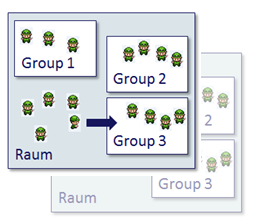
\includegraphics{graphiken/konzeptskizze.png}%
\caption{Konzeptskizze von Raum, Gruppen und Mitgliedern (Quelle: Eigene Darstellung)}%
\label{konzeptskizze}%
\end{figure}

Die Bewegung der eigenen Figur kann dabei mit den Pfeiltasten einer Tastatur oder mit Hilfe des Fingers per Drag'n'Drop auf mobilen Endgeräten erfolgen. Die technische Details zur Realisierung werden im Kapitel \ref{architektur_technologie} näher erläutert. 
\newline\newline
Des Weiteren existiert pro Raum ein Chatfenster, in dem die Mitglieder sich unterhalten können. Mögliche Gesprächsthemen wären bspw. die Findung eines Gruppennamens, der Gruppenzusammensetzung oder die Aufgaben einer möglichen Gruppe. Da keine persistente Speicherung der Gruppen sowie deren Mitglieder nach Verlassen des Raumes vorgesehen ist, ist eine Exportfunktion der angezeigten Gruppeninformationen vorhanden. Aktuell ist jedoch nicht sichergestellt, dass jeweils ein konsistenter Zustand exportiert wird.